% Options for packages loaded elsewhere
\PassOptionsToPackage{unicode}{hyperref}
\PassOptionsToPackage{hyphens}{url}
%
\documentclass[
]{article}
\usepackage{amsmath,amssymb}
\usepackage{iftex}
\ifPDFTeX
  \usepackage[T1]{fontenc}
  \usepackage[utf8]{inputenc}
  \usepackage{textcomp} % provide euro and other symbols
\else % if luatex or xetex
  \usepackage{unicode-math} % this also loads fontspec
  \defaultfontfeatures{Scale=MatchLowercase}
  \defaultfontfeatures[\rmfamily]{Ligatures=TeX,Scale=1}
\fi
\usepackage{lmodern}
\ifPDFTeX\else
  % xetex/luatex font selection
\fi
% Use upquote if available, for straight quotes in verbatim environments
\IfFileExists{upquote.sty}{\usepackage{upquote}}{}
\IfFileExists{microtype.sty}{% use microtype if available
  \usepackage[]{microtype}
  \UseMicrotypeSet[protrusion]{basicmath} % disable protrusion for tt fonts
}{}
\makeatletter
\@ifundefined{KOMAClassName}{% if non-KOMA class
  \IfFileExists{parskip.sty}{%
    \usepackage{parskip}
  }{% else
    \setlength{\parindent}{0pt}
    \setlength{\parskip}{6pt plus 2pt minus 1pt}}
}{% if KOMA class
  \KOMAoptions{parskip=half}}
\makeatother
\usepackage{xcolor}
\usepackage[margin=1in]{geometry}
\usepackage{color}
\usepackage{fancyvrb}
\newcommand{\VerbBar}{|}
\newcommand{\VERB}{\Verb[commandchars=\\\{\}]}
\DefineVerbatimEnvironment{Highlighting}{Verbatim}{commandchars=\\\{\}}
% Add ',fontsize=\small' for more characters per line
\usepackage{framed}
\definecolor{shadecolor}{RGB}{248,248,248}
\newenvironment{Shaded}{\begin{snugshade}}{\end{snugshade}}
\newcommand{\AlertTok}[1]{\textcolor[rgb]{0.94,0.16,0.16}{#1}}
\newcommand{\AnnotationTok}[1]{\textcolor[rgb]{0.56,0.35,0.01}{\textbf{\textit{#1}}}}
\newcommand{\AttributeTok}[1]{\textcolor[rgb]{0.13,0.29,0.53}{#1}}
\newcommand{\BaseNTok}[1]{\textcolor[rgb]{0.00,0.00,0.81}{#1}}
\newcommand{\BuiltInTok}[1]{#1}
\newcommand{\CharTok}[1]{\textcolor[rgb]{0.31,0.60,0.02}{#1}}
\newcommand{\CommentTok}[1]{\textcolor[rgb]{0.56,0.35,0.01}{\textit{#1}}}
\newcommand{\CommentVarTok}[1]{\textcolor[rgb]{0.56,0.35,0.01}{\textbf{\textit{#1}}}}
\newcommand{\ConstantTok}[1]{\textcolor[rgb]{0.56,0.35,0.01}{#1}}
\newcommand{\ControlFlowTok}[1]{\textcolor[rgb]{0.13,0.29,0.53}{\textbf{#1}}}
\newcommand{\DataTypeTok}[1]{\textcolor[rgb]{0.13,0.29,0.53}{#1}}
\newcommand{\DecValTok}[1]{\textcolor[rgb]{0.00,0.00,0.81}{#1}}
\newcommand{\DocumentationTok}[1]{\textcolor[rgb]{0.56,0.35,0.01}{\textbf{\textit{#1}}}}
\newcommand{\ErrorTok}[1]{\textcolor[rgb]{0.64,0.00,0.00}{\textbf{#1}}}
\newcommand{\ExtensionTok}[1]{#1}
\newcommand{\FloatTok}[1]{\textcolor[rgb]{0.00,0.00,0.81}{#1}}
\newcommand{\FunctionTok}[1]{\textcolor[rgb]{0.13,0.29,0.53}{\textbf{#1}}}
\newcommand{\ImportTok}[1]{#1}
\newcommand{\InformationTok}[1]{\textcolor[rgb]{0.56,0.35,0.01}{\textbf{\textit{#1}}}}
\newcommand{\KeywordTok}[1]{\textcolor[rgb]{0.13,0.29,0.53}{\textbf{#1}}}
\newcommand{\NormalTok}[1]{#1}
\newcommand{\OperatorTok}[1]{\textcolor[rgb]{0.81,0.36,0.00}{\textbf{#1}}}
\newcommand{\OtherTok}[1]{\textcolor[rgb]{0.56,0.35,0.01}{#1}}
\newcommand{\PreprocessorTok}[1]{\textcolor[rgb]{0.56,0.35,0.01}{\textit{#1}}}
\newcommand{\RegionMarkerTok}[1]{#1}
\newcommand{\SpecialCharTok}[1]{\textcolor[rgb]{0.81,0.36,0.00}{\textbf{#1}}}
\newcommand{\SpecialStringTok}[1]{\textcolor[rgb]{0.31,0.60,0.02}{#1}}
\newcommand{\StringTok}[1]{\textcolor[rgb]{0.31,0.60,0.02}{#1}}
\newcommand{\VariableTok}[1]{\textcolor[rgb]{0.00,0.00,0.00}{#1}}
\newcommand{\VerbatimStringTok}[1]{\textcolor[rgb]{0.31,0.60,0.02}{#1}}
\newcommand{\WarningTok}[1]{\textcolor[rgb]{0.56,0.35,0.01}{\textbf{\textit{#1}}}}
\usepackage{longtable,booktabs,array}
\usepackage{calc} % for calculating minipage widths
% Correct order of tables after \paragraph or \subparagraph
\usepackage{etoolbox}
\makeatletter
\patchcmd\longtable{\par}{\if@noskipsec\mbox{}\fi\par}{}{}
\makeatother
% Allow footnotes in longtable head/foot
\IfFileExists{footnotehyper.sty}{\usepackage{footnotehyper}}{\usepackage{footnote}}
\makesavenoteenv{longtable}
\usepackage{graphicx}
\makeatletter
\def\maxwidth{\ifdim\Gin@nat@width>\linewidth\linewidth\else\Gin@nat@width\fi}
\def\maxheight{\ifdim\Gin@nat@height>\textheight\textheight\else\Gin@nat@height\fi}
\makeatother
% Scale images if necessary, so that they will not overflow the page
% margins by default, and it is still possible to overwrite the defaults
% using explicit options in \includegraphics[width, height, ...]{}
\setkeys{Gin}{width=\maxwidth,height=\maxheight,keepaspectratio}
% Set default figure placement to htbp
\makeatletter
\def\fps@figure{htbp}
\makeatother
\setlength{\emergencystretch}{3em} % prevent overfull lines
\providecommand{\tightlist}{%
  \setlength{\itemsep}{0pt}\setlength{\parskip}{0pt}}
\setcounter{secnumdepth}{-\maxdimen} % remove section numbering
\ifLuaTeX
  \usepackage{selnolig}  % disable illegal ligatures
\fi
\usepackage{bookmark}
\IfFileExists{xurl.sty}{\usepackage{xurl}}{} % add URL line breaks if available
\urlstyle{same}
\hypersetup{
  pdfauthor={Sangho Lee},
  hidelinks,
  pdfcreator={LaTeX via pandoc}}

\author{Sangho Lee}
\date{7/12/2024}

\begin{document}

\section{Belkin - Case Study: eCommerce Data Analyst Hiring Process
{[}Sangho
Lee{]}}\label{belkin---case-study-ecommerce-data-analyst-hiring-process-sangho-lee}

I explored eCommerce analytics with a case study on Belkin's performance
on the Amazon Marketplace. Using the provided data, I analyzed Belkin's
metrics to offer actionable insights, focusing on key indicators for
revenue growth, investment opportunities, and recommendations for
improvement. Additionally, I demonstrated these insights through an
interactive dashboard and discussed strategies for automating data
processing on this website.

\subsubsection{Summary of the Regression
model}\label{summary-of-the-regression-model}

Based on our findings from questions 1 and 2, we have examined the
quality of the data, created a regression model, and identified the key
drivers of revenue by analyzing the p-values and coefficients to
determine the most significant predictors.

\begin{Shaded}
\begin{Highlighting}[]
\CommentTok{\# Show the regression model}
\FunctionTok{summary}\NormalTok{(model)}
\end{Highlighting}
\end{Shaded}

\begin{verbatim}
## 
## Call:
## lm(formula = ordered_revenue_amount ~ ., data = data_train)
## 
## Residuals:
##    Min     1Q Median     3Q    Max 
## -77579   -612   -189    396 118367 
## 
## Coefficients: (2 not defined because of singularities)
##                     Estimate   Std. Error t value            Pr(>|t|)    
## (Intercept)      5867.940130 14735.909116   0.398              0.6905    
## week_ending        -0.364153     0.743986  -0.489              0.6245    
## asin                0.011511     0.001368   8.416 <0.0000000000000002 ***
## ordered_units      20.675258     0.205555 100.583 <0.0000000000000002 ***
## asp                31.373871     0.967078  32.442 <0.0000000000000002 ***
## category.a         30.402476   106.148560   0.286              0.7746    
## category.b         -3.528137   106.208459  -0.033              0.9735    
## category.c        180.248411   106.282564   1.696              0.0899 .  
## category.d                NA           NA      NA                  NA    
## subcategory.aa   -106.172324   118.636310  -0.895              0.3708    
## subcategory.bb    164.342191   118.622853   1.385              0.1660    
## subcategory.cc      5.252084   118.383693   0.044              0.9646    
## subcategory.dd    -21.019948   118.537029  -0.177              0.8593    
## subcategory.ee            NA           NA      NA                  NA    
## marketing_spend    -0.034668     0.032283  -1.074              0.2829    
## views               0.079425     0.067711   1.173              0.2408    
## ---
## Signif. codes:  0 '***' 0.001 '**' 0.01 '*' 0.05 '.' 0.1 ' ' 1
## 
## Residual standard error: 4067 on 11762 degrees of freedom
## Multiple R-squared:  0.485,  Adjusted R-squared:  0.4845 
## F-statistic: 852.2 on 13 and 11762 DF,  p-value: < 0.00000000000000022
\end{verbatim}

From this model, we found that the most significant predictors of
revenue are:

\begin{itemize}
\item
  Number of units ordered (ordered\_units): Coefficient = 20.67. This
  indicates that for each additional unit ordered, revenue increases by
  \$20.67 (p-value \textless{} 0.00002).
\item
  Average selling price (asp): Coefficient = 31.37. This means that for
  each \$1 increase in the average selling price, revenue increases by
  \$31.37 (p-value \textless{} 0.00002).
\item
  Product identification number (asin): With a p-value of 0.00002, this
  predictor is also significant.
\end{itemize}

Although there are other predictors with high absolute coefficients,
they are not as significant in terms of the p-value, indicating that
they are not as reliable in this model.

Based on this rationale, I have made the following recommendations for
actions to improve revenue:

\begin{enumerate}
\def\labelenumi{\arabic{enumi}.}
\tightlist
\item
  Focus on Increasing Units Sold
\end{enumerate}

\begin{itemize}
\item
  Rationale: The number of units sold (ordered\_units) is the most
  significant predictor of revenue, with a coefficient of 20.671226 and
  a very low p-value (\textless{} 0.0000000000000002). This strong
  positive relationship indicates that increasing the number of units
  sold will significantly boost revenue.
\item
  Action: Implement strategies to increase units sold, such as
  promotional campaigns, discounts for bulk purchases, and improved
  product availability. Enhance distribution channels to ensure products
  are always in stock and accessible to customers.
\end{itemize}

\begin{enumerate}
\def\labelenumi{\arabic{enumi}.}
\setcounter{enumi}{1}
\tightlist
\item
  Optimize Average Selling Price (ASP)
\end{enumerate}

\begin{itemize}
\item
  Rationale: The average selling price (asp) also has a significant
  positive impact on revenue, with a coefficient of 31.411177 and a very
  low p-value (\textless{} 0.0000000000000002). Higher ASP contributes
  to higher revenue.
\item
  Action: Evaluate the pricing strategy to find an optimal balance that
  maximizes revenue without reducing demand. Consider value-based
  pricing, premium pricing for high-demand products, and periodic price
  adjustments based on market trends and competitor pricing.
\end{itemize}

\begin{enumerate}
\def\labelenumi{\arabic{enumi}.}
\setcounter{enumi}{2}
\tightlist
\item
  Leverage Product Identification (ASIN)
\end{enumerate}

\begin{itemize}
\item
  Rationale: The asin variable, which represents product identification,
  has a significant positive coefficient of 0.011480 with a very low
  p-value (\textless{} 0.0000000000000002). This suggests that certain
  products inherently drive higher revenue.
\item
  Action: Identify and prioritize products with high revenue potential
  based on their ASINs. Focus marketing and promotional efforts on these
  high-performing products. Additionally, analyze characteristics of
  these high-revenue ASINs to replicate their success across other
  products.
\end{itemize}

Now that we have identified the key drivers according to the model, we
have redesigned it using only the significant variables to enhance its
strength.

\begin{Shaded}
\begin{Highlighting}[]
\CommentTok{\# Show the refiend model that I created in the previous question}
\FunctionTok{summary}\NormalTok{(refined\_model)}
\end{Highlighting}
\end{Shaded}

\begin{verbatim}
## 
## Call:
## lm(formula = ordered_revenue_amount ~ asin + ordered_units + 
##     asp, data = data_train)
## 
## Residuals:
##    Min     1Q Median     3Q    Max 
## -77609   -597   -203    387 118636 
## 
## Coefficients:
##                   Estimate   Std. Error t value            Pr(>|t|)    
## (Intercept)   -1306.511753    94.473524 -13.829 <0.0000000000000002 ***
## asin              0.011480     0.001364   8.414 <0.0000000000000002 ***
## ordered_units    20.671226     0.205513 100.584 <0.0000000000000002 ***
## asp              31.411177     0.966556  32.498 <0.0000000000000002 ***
## ---
## Signif. codes:  0 '***' 0.001 '**' 0.01 '*' 0.05 '.' 0.1 ' ' 1
## 
## Residual standard error: 4068 on 11772 degrees of freedom
## Multiple R-squared:  0.4845, Adjusted R-squared:  0.4844 
## F-statistic:  3688 on 3 and 11772 DF,  p-value: < 0.00000000000000022
\end{verbatim}

We then added the predicted\_revenue column to the dataset. With this,
we can now categorize the areas that overperformed and underperformed
according to the model's predictions.

\begin{Shaded}
\begin{Highlighting}[]
\NormalTok{predicted\_revenue\_table}
\end{Highlighting}
\end{Shaded}

\begin{longtable}[]{@{}
  >{\raggedleft\arraybackslash}p{(\columnwidth - 14\tabcolsep) * \real{0.1154}}
  >{\raggedleft\arraybackslash}p{(\columnwidth - 14\tabcolsep) * \real{0.0577}}
  >{\raggedleft\arraybackslash}p{(\columnwidth - 14\tabcolsep) * \real{0.2212}}
  >{\raggedleft\arraybackslash}p{(\columnwidth - 14\tabcolsep) * \real{0.1346}}
  >{\raggedleft\arraybackslash}p{(\columnwidth - 14\tabcolsep) * \real{0.0865}}
  >{\raggedleft\arraybackslash}p{(\columnwidth - 14\tabcolsep) * \real{0.1538}}
  >{\raggedleft\arraybackslash}p{(\columnwidth - 14\tabcolsep) * \real{0.0577}}
  >{\raggedleft\arraybackslash}p{(\columnwidth - 14\tabcolsep) * \real{0.1731}}@{}}
\toprule\noalign{}
\begin{minipage}[b]{\linewidth}\raggedleft
week\_ending
\end{minipage} & \begin{minipage}[b]{\linewidth}\raggedleft
asin
\end{minipage} & \begin{minipage}[b]{\linewidth}\raggedleft
ordered\_revenue\_amount
\end{minipage} & \begin{minipage}[b]{\linewidth}\raggedleft
ordered\_units
\end{minipage} & \begin{minipage}[b]{\linewidth}\raggedleft
asp
\end{minipage} & \begin{minipage}[b]{\linewidth}\raggedleft
marketing\_spend
\end{minipage} & \begin{minipage}[b]{\linewidth}\raggedleft
views
\end{minipage} & \begin{minipage}[b]{\linewidth}\raggedleft
predicted\_revenue
\end{minipage} \\
\midrule\noalign{}
\endhead
\bottomrule\noalign{}
\endlastfoot
19728 & 99345 & 1902.66 & 95 & 20.02800 & 3741 & 111 & 2426.7939 \\
19728 & 91686 & 224.15 & 12 & 18.67917 & 2309 & 185 & 580.7918 \\
19728 & 90798 & 437.74 & 9 & 48.63778 & 4781 & 253 & 1449.6195 \\
19728 & 28305 & 4.95 & 1 & 4.95000 & 1643 & 1069 & -805.4265 \\
19728 & 52947 & 13.49 & 1 & 13.49000 & 3206 & 347 & -254.2959 \\
19728 & 40959 & 13064.52 & 597 & 21.88362 & 1292 & 323 & 12191.7913 \\
19728 & 57942 & 612.19 & 34 & 18.00559 & 3432 & 1876 & 627.0348 \\
19728 & 58053 & 602.36 & 44 & 13.69000 & 1284 & 408 & 699.4636 \\
19728 & 60495 & 280.14 & 6 & 46.69000 & 3930 & 1156 & 978.5589 \\
19728 & 59385 & 1816.13 & 69 & 26.32072 & 4519 & 1673 & 1628.2810 \\
\end{longtable}

Then we moved on to the second question to dive deeper into which
specific products to focus on. Before visualizing the data, I explained
why we should focus on predicted revenue from the model instead of
relying solely on actual sales data.

\subparagraph{Benefits of Utilizing Model Prediction Data Instead of
Relying on Actual Sales
Data}\label{benefits-of-utilizing-model-prediction-data-instead-of-relying-on-actual-sales-data}

\begin{itemize}
\tightlist
\item
  Identify potential issues like stock shortages.
\item
  Optimize marketing strategies.
\item
  Adjust pricing to match market demand.
\item
  Improve product listings to enhance conversions.
\item
  Prepare for seasonal demand.
\item
  Estimate potential success for new product launches.
\end{itemize}

This approach is crucial for identifying potential issues like stock
shortages, optimizing marketing strategies, adjusting pricing to match
market demand, improving product listings to enhance conversions,
preparing for seasonal demand, and estimating potential success for new
product launches.

\begin{Shaded}
\begin{Highlighting}[]
\CommentTok{\# Show the plot of Actual vs. Predicted Revenue}
\NormalTok{plot\_actual\_vs\_predicted\_revenue}
\end{Highlighting}
\end{Shaded}

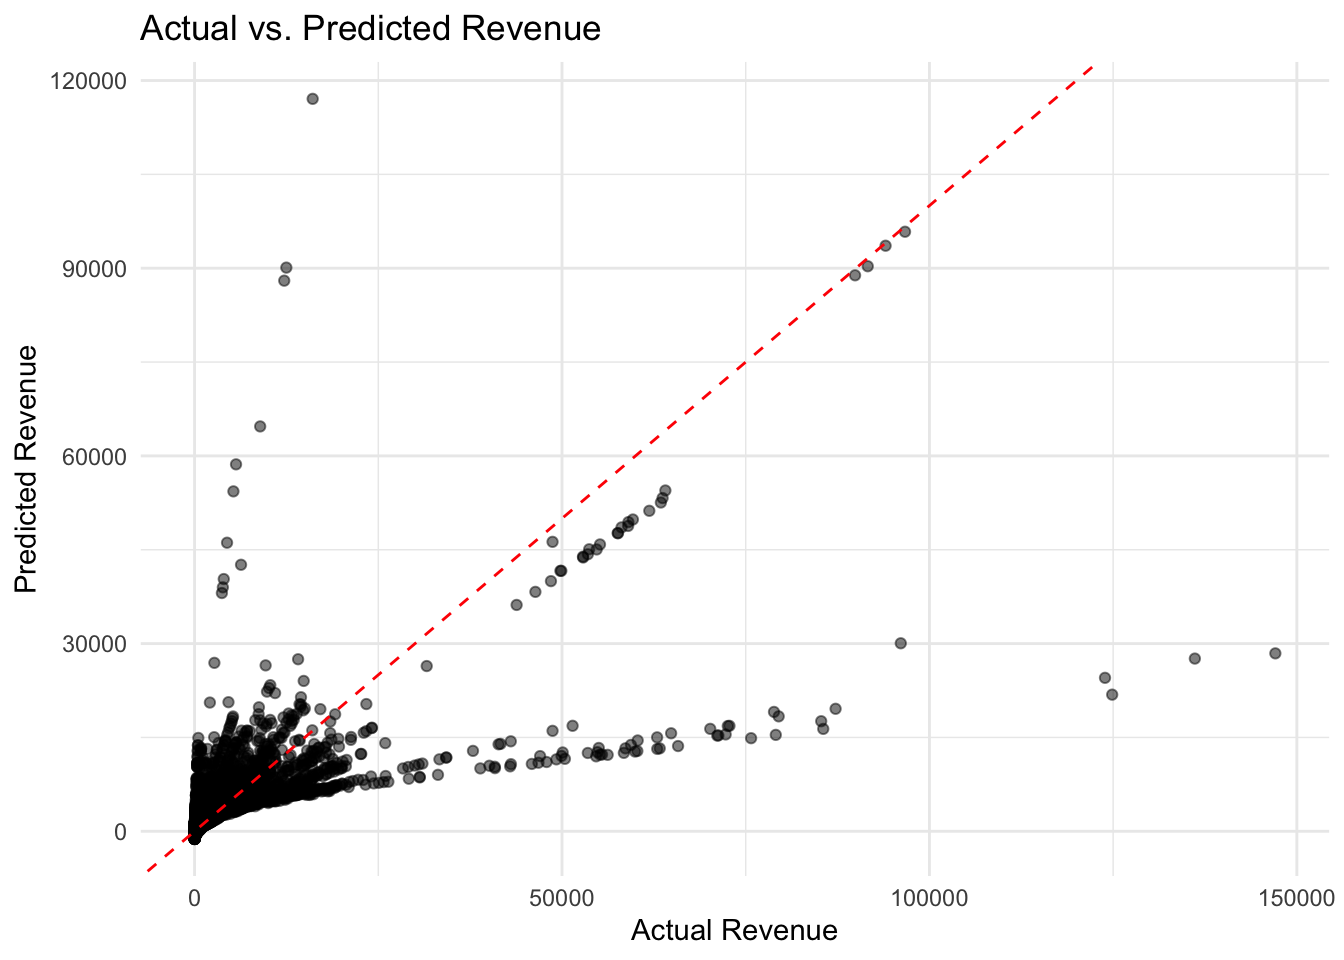
\includegraphics{Belkin_case_study_files/figure-latex/unnamed-chunk-14-1.pdf}

Looking at this plot, we were able to identify areas where actual
revenue was higher or lower than predicted revenue. This information
helps us focus on specific products that may require further analysis or
action to improve sales performance.

To pinpoint the specific products that overperformed or underperformed,
we set a threshold for the outliers in the plot. The identified products
are shown in the visualization below.

\begin{Shaded}
\begin{Highlighting}[]
\CommentTok{\# Show the plot of Actual vs. Predicted Revenue with Critical Score by Actual Revenue}
\NormalTok{plot\_actual\_vs\_predicted\_revenue\_critical}
\end{Highlighting}
\end{Shaded}

\begin{center}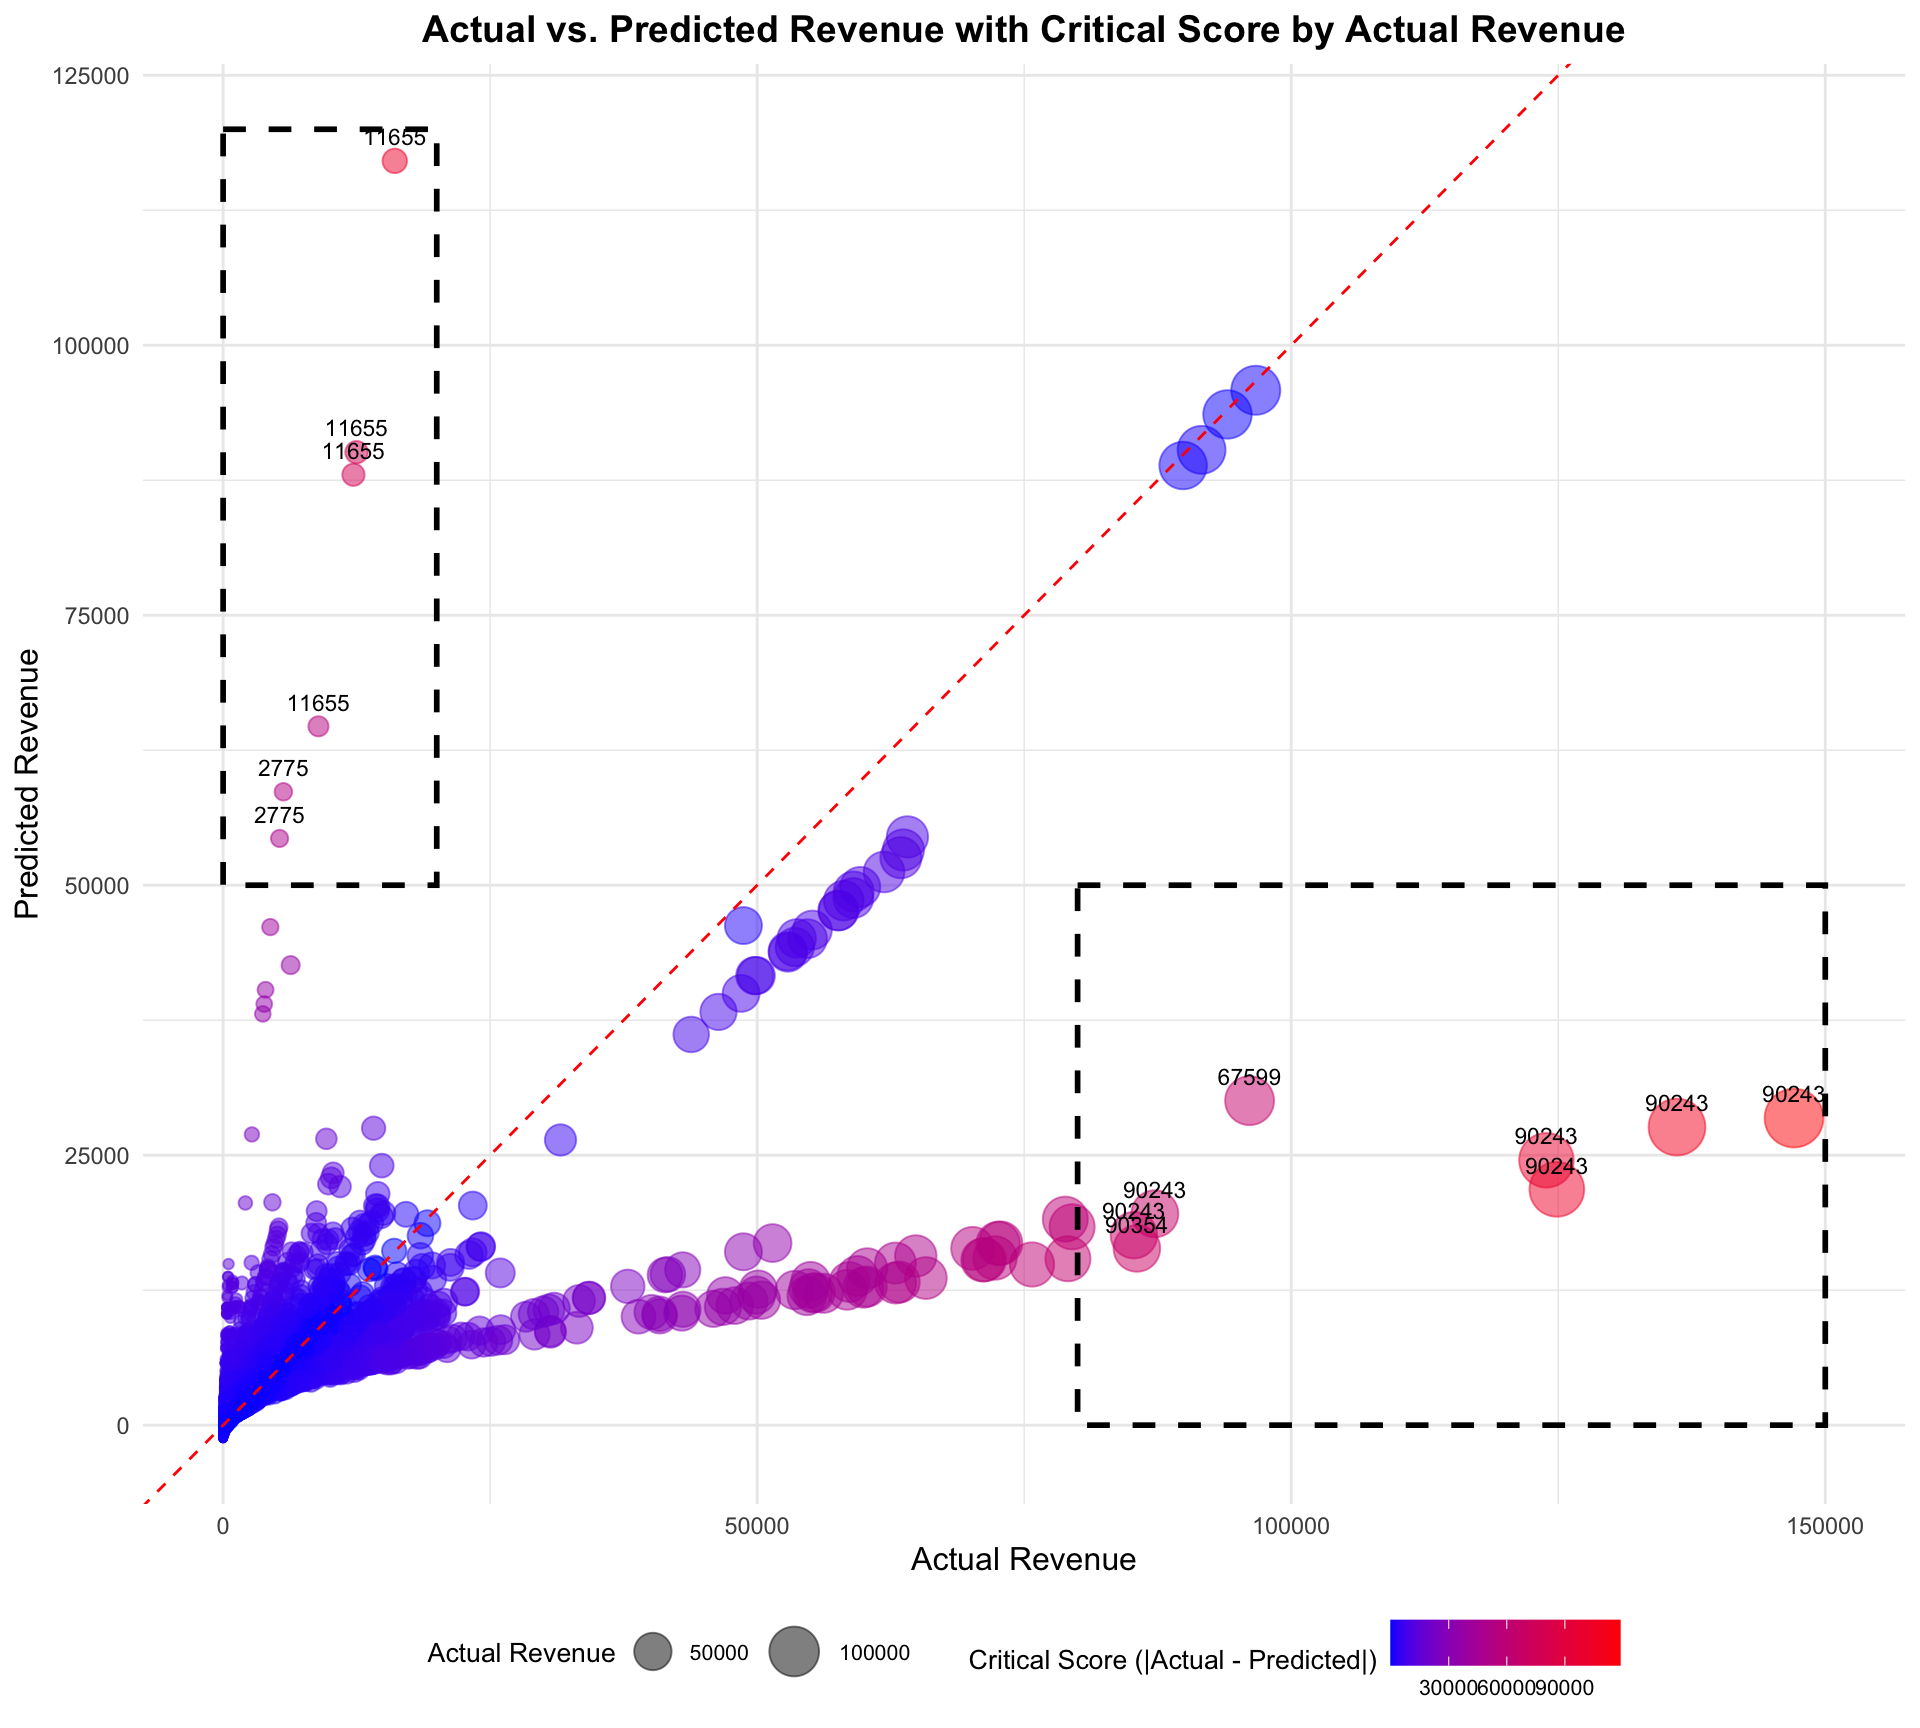
\includegraphics{Belkin_case_study_files/figure-latex/unnamed-chunk-16-1} \end{center}

Next, we categorized the products into two focus areas based on the plot
criteria:

\begin{itemize}
\tightlist
\item
  Focus Area 1: Products with high predicted revenue but low actual
  revenue. These products likely have potential, but something may be
  missing to maximize their profit.
\item
  Focus Area 2: Products with low predicted revenue but high actual
  revenue. We need to investigate why these products are performing
  better than predicted. Understanding the reasons behind their success
  can help replicate it for other products or minimize risks in the
  future.
\end{itemize}

\begin{Shaded}
\begin{Highlighting}[]
\NormalTok{segmented\_data\_table}
\end{Highlighting}
\end{Shaded}

\begin{longtable}[]{@{}
  >{\raggedleft\arraybackslash}p{(\columnwidth - 4\tabcolsep) * \real{0.0458}}
  >{\raggedright\arraybackslash}p{(\columnwidth - 4\tabcolsep) * \real{0.3359}}
  >{\raggedright\arraybackslash}p{(\columnwidth - 4\tabcolsep) * \real{0.6183}}@{}}
\toprule\noalign{}
\begin{minipage}[b]{\linewidth}\raggedleft
asin
\end{minipage} & \begin{minipage}[b]{\linewidth}\raggedright
focus\_area
\end{minipage} & \begin{minipage}[b]{\linewidth}\raggedright
check\_items
\end{minipage} \\
\midrule\noalign{}
\endhead
\bottomrule\noalign{}
\endlastfoot
2775 & Focus Area 1 (High Prediction, Low Revenue) & Investigate Stock
Levels, Enhance Marketing Strategies, Improve Product Listings \\
11655 & Focus Area 1 (High Prediction, Low Revenue) & Investigate Stock
Levels, Enhance Marketing Strategies, Improve Product Listings \\
67599 & Focus Area 2 (Low Prediction, High Revenue) & Examine Sales
Trends, Optimize Stock Management, Replicate Success \\
90243 & Focus Area 2 (Low Prediction, High Revenue) & Examine Sales
Trends, Optimize Stock Management, Replicate Success \\
90354 & Focus Area 2 (Low Prediction, High Revenue) & Examine Sales
Trends, Optimize Stock Management, Replicate Success \\
\end{longtable}

\subsubsection{Conclusion}\label{conclusion}

Based on the analysis of this dataset, we identified the key drivers by
examining statistical indicators from the model, pinpointed products
that are overperforming or underperforming, and segmented the products
into two focus areas for further investigation. Using this approach, I
recommend investing further in the following five products to maximize
revenue by either boosting sales or preventing revenue decline.

In this analysis, I will perform additional descriptive analysis to
extract insights from the given data.

\subsubsection{1. Revenue vs.~Marketing Spend
vs.~Views}\label{revenue-vs.-marketing-spend-vs.-views}

\begin{Shaded}
\begin{Highlighting}[]
\CommentTok{\# Create scatter plot of Revenue vs Marketing Spend}
\NormalTok{p1 }\OtherTok{\textless{}{-}} \FunctionTok{ggplot}\NormalTok{(belkin\_data, }\FunctionTok{aes}\NormalTok{(}\AttributeTok{x =}\NormalTok{ marketing\_spend, }\AttributeTok{y =}\NormalTok{ ordered\_revenue\_amount, }\AttributeTok{color =}\NormalTok{ asp, }\AttributeTok{size =}\NormalTok{ views)) }\SpecialCharTok{+}
  \FunctionTok{geom\_point}\NormalTok{(}\AttributeTok{alpha =} \FloatTok{0.6}\NormalTok{) }\SpecialCharTok{+}
  \FunctionTok{scale\_color\_gradient}\NormalTok{(}\AttributeTok{low =} \StringTok{"blue"}\NormalTok{, }\AttributeTok{high =} \StringTok{"red"}\NormalTok{) }\SpecialCharTok{+}
  \FunctionTok{labs}\NormalTok{(}\AttributeTok{title =} \StringTok{"Revenue vs. Marketing Spend with ASP"}\NormalTok{, }\AttributeTok{x =} \StringTok{"Marketing Spend ($)"}\NormalTok{, }\AttributeTok{y =} \StringTok{"Revenue ($)"}\NormalTok{, }\AttributeTok{color =} \StringTok{"ASP ($)"}\NormalTok{) }\SpecialCharTok{+}
  \FunctionTok{theme\_minimal}\NormalTok{()}

\CommentTok{\# Create scatter plot of Revenue vs. Views, color{-}coded by Marketing Spend and size by ASP}
\NormalTok{p2 }\OtherTok{\textless{}{-}} \FunctionTok{ggplot}\NormalTok{(belkin\_data, }\FunctionTok{aes}\NormalTok{(}\AttributeTok{x =}\NormalTok{ views, }\AttributeTok{y =}\NormalTok{ ordered\_revenue\_amount, }\AttributeTok{color =}\NormalTok{ marketing\_spend, }\AttributeTok{size =}\NormalTok{ asp)) }\SpecialCharTok{+}
  \FunctionTok{geom\_point}\NormalTok{(}\AttributeTok{alpha =} \FloatTok{0.7}\NormalTok{) }\SpecialCharTok{+}
  \FunctionTok{scale\_color\_gradient}\NormalTok{(}\AttributeTok{low =} \StringTok{"blue"}\NormalTok{, }\AttributeTok{high =} \StringTok{"red"}\NormalTok{) }\SpecialCharTok{+}
  \FunctionTok{labs}\NormalTok{(}\AttributeTok{title =} \StringTok{"Revenue vs. Views with Marketing Spend and ASP"}\NormalTok{,}
       \AttributeTok{x =} \StringTok{"Views"}\NormalTok{,}
       \AttributeTok{y =} \StringTok{"Revenue ($)"}\NormalTok{,}
       \AttributeTok{color =} \StringTok{"Marketing Spend ($)"}\NormalTok{,}
       \AttributeTok{size =} \StringTok{"ASP ($)"}\NormalTok{) }\SpecialCharTok{+}
  \FunctionTok{theme\_minimal}\NormalTok{() }\SpecialCharTok{+}
  \FunctionTok{theme}\NormalTok{(}\AttributeTok{legend.position =} \StringTok{"right"}\NormalTok{,}
        \AttributeTok{plot.title =} \FunctionTok{element\_text}\NormalTok{(}\AttributeTok{hjust =} \FloatTok{0.5}\NormalTok{, }\AttributeTok{size =} \DecValTok{14}\NormalTok{, }\AttributeTok{face =} \StringTok{"bold"}\NormalTok{),}
        \AttributeTok{axis.title.x =} \FunctionTok{element\_text}\NormalTok{(}\AttributeTok{size =} \DecValTok{12}\NormalTok{),}
        \AttributeTok{axis.title.y =} \FunctionTok{element\_text}\NormalTok{(}\AttributeTok{size =} \DecValTok{12}\NormalTok{),}
        \AttributeTok{legend.title =} \FunctionTok{element\_text}\NormalTok{(}\AttributeTok{size =} \DecValTok{10}\NormalTok{),}
        \AttributeTok{legend.text =} \FunctionTok{element\_text}\NormalTok{(}\AttributeTok{size =} \DecValTok{8}\NormalTok{))}

\CommentTok{\# Combine the two plots into one screen}
\NormalTok{combined\_plot }\OtherTok{\textless{}{-}}\NormalTok{ p1 }\SpecialCharTok{+}\NormalTok{ p2 }\SpecialCharTok{+} \FunctionTok{plot\_layout}\NormalTok{(}\AttributeTok{ncol =} \DecValTok{1}\NormalTok{, }\AttributeTok{heights =} \FunctionTok{c}\NormalTok{(}\DecValTok{1}\NormalTok{, }\DecValTok{1}\NormalTok{))}

\CommentTok{\# Display the combined plot}
\NormalTok{combined\_plot}
\end{Highlighting}
\end{Shaded}

\includegraphics{Belkin_case_study_files/figure-latex/unnamed-chunk-20-1.pdf}

\paragraph{Revenue vs.~Marketing
Spend:}\label{revenue-vs.-marketing-spend}

\begin{itemize}
\tightlist
\item
  Spread Across Spend: The marketing spend is distributed across the
  entire range from \$0 to \$5000, indicating a diverse allocation of
  marketing budgets across different products.
\item
  Revenue Distribution: Revenue is mostly clustered at lower values,
  even with varying marketing spend levels. This suggests that high
  marketing spend does not always translate to higher revenue.
\item
  ASP Impact: ASP ranges from \$80 to \$180, with clusters (in purplish
  color) around higher revenue values.
\end{itemize}

\paragraph{Revenue vs.~Views:}\label{revenue-vs.-views}

\begin{itemize}
\tightlist
\item
  Views Distribution: The views range from 0 to 2000, showing that
  product visibility varies widely.
\item
  Revenue Clustering: Similar to marketing spend, revenue is clustered
  at lower values regardless of the number of views
\item
  Marketing Spend Clustering: Products with higher marketing spend are
  clustered around lower revenue values, indicating that increased
  marketing spend does not always lead to higher revenue.
\end{itemize}

\paragraph{Key Takeaways:}\label{key-takeaways}

\begin{itemize}
\tightlist
\item
  Optimize Marketing Spend: Since revenue does not consistently increase
  with higher marketing spend, it's important to evaluate the
  effectiveness of marketing campaigns and reallocate budget towards
  more impactful strategies.
\item
  More Views Generally Lead to More Revenue: Products with higher views
  tend to generate more revenue, suggesting that increasing product
  visibility can positively impact sales.
\end{itemize}

\subsubsection{2. Revenue Over Time vs.~Views Over
Time}\label{revenue-over-time-vs.-views-over-time}

\begin{Shaded}
\begin{Highlighting}[]
\CommentTok{\# Line plot of Revenue over Time}
\NormalTok{t1 }\OtherTok{\textless{}{-}}\NormalTok{ belkin\_data }\SpecialCharTok{\%\textgreater{}\%}
  \FunctionTok{mutate}\NormalTok{(}\AttributeTok{week\_ending =} \FunctionTok{as.Date}\NormalTok{(week\_ending)) }\SpecialCharTok{\%\textgreater{}\%}
  \FunctionTok{group\_by}\NormalTok{(week\_ending) }\SpecialCharTok{\%\textgreater{}\%}
  \FunctionTok{summarise}\NormalTok{(}\AttributeTok{total\_revenue =} \FunctionTok{sum}\NormalTok{(ordered\_revenue\_amount)) }\SpecialCharTok{\%\textgreater{}\%}
  \FunctionTok{ggplot}\NormalTok{(}\FunctionTok{aes}\NormalTok{(}\AttributeTok{x =}\NormalTok{ week\_ending, }\AttributeTok{y =}\NormalTok{ total\_revenue)) }\SpecialCharTok{+}
  \FunctionTok{geom\_line}\NormalTok{(}\AttributeTok{color =} \StringTok{"blue"}\NormalTok{) }\SpecialCharTok{+}
  \FunctionTok{labs}\NormalTok{(}\AttributeTok{title =} \StringTok{"Revenue Over Time"}\NormalTok{, }\AttributeTok{x =} \StringTok{"Week Ending"}\NormalTok{, }\AttributeTok{y =} \StringTok{"Total Revenue ($)"}\NormalTok{) }\SpecialCharTok{+}
  \FunctionTok{theme\_minimal}\NormalTok{()}\SpecialCharTok{+}
    \FunctionTok{theme}\NormalTok{(}\AttributeTok{plot.title =} \FunctionTok{element\_text}\NormalTok{(}\AttributeTok{hjust =} \FloatTok{0.5}\NormalTok{, }\AttributeTok{size =} \DecValTok{14}\NormalTok{, }\AttributeTok{face =} \StringTok{"bold"}\NormalTok{),}
        \AttributeTok{axis.title.x =} \FunctionTok{element\_text}\NormalTok{(}\AttributeTok{size =} \DecValTok{12}\NormalTok{),}
        \AttributeTok{axis.title.y =} \FunctionTok{element\_text}\NormalTok{(}\AttributeTok{size =} \DecValTok{12}\NormalTok{))}

\CommentTok{\# Line plot of Views Over Time}
\NormalTok{t2 }\OtherTok{\textless{}{-}}\NormalTok{ belkin\_data }\SpecialCharTok{\%\textgreater{}\%}
  \FunctionTok{mutate}\NormalTok{(}\AttributeTok{week\_ending =} \FunctionTok{as.Date}\NormalTok{(week\_ending)) }\SpecialCharTok{\%\textgreater{}\%}
  \FunctionTok{group\_by}\NormalTok{(week\_ending) }\SpecialCharTok{\%\textgreater{}\%}
  \FunctionTok{summarise}\NormalTok{(}\AttributeTok{total\_views =} \FunctionTok{sum}\NormalTok{(views)) }\SpecialCharTok{\%\textgreater{}\%}
  \FunctionTok{ggplot}\NormalTok{(}\FunctionTok{aes}\NormalTok{(}\AttributeTok{x =}\NormalTok{ week\_ending, }\AttributeTok{y =}\NormalTok{ total\_views)) }\SpecialCharTok{+}
  \FunctionTok{geom\_line}\NormalTok{(}\AttributeTok{color =} \StringTok{"red"}\NormalTok{) }\SpecialCharTok{+}
  \FunctionTok{labs}\NormalTok{(}\AttributeTok{title =} \StringTok{"Views Over Time"}\NormalTok{,}
       \AttributeTok{x =} \StringTok{"Week Ending"}\NormalTok{,}
       \AttributeTok{y =} \StringTok{"Total Views"}\NormalTok{) }\SpecialCharTok{+}
  \FunctionTok{theme\_minimal}\NormalTok{() }\SpecialCharTok{+}
  \FunctionTok{theme}\NormalTok{(}\AttributeTok{plot.title =} \FunctionTok{element\_text}\NormalTok{(}\AttributeTok{hjust =} \FloatTok{0.5}\NormalTok{, }\AttributeTok{size =} \DecValTok{14}\NormalTok{, }\AttributeTok{face =} \StringTok{"bold"}\NormalTok{),}
        \AttributeTok{axis.title.x =} \FunctionTok{element\_text}\NormalTok{(}\AttributeTok{size =} \DecValTok{12}\NormalTok{),}
        \AttributeTok{axis.title.y =} \FunctionTok{element\_text}\NormalTok{(}\AttributeTok{size =} \DecValTok{12}\NormalTok{))}

\NormalTok{combined\_plot\_2 }\OtherTok{\textless{}{-}}\NormalTok{ t1 }\SpecialCharTok{/}\NormalTok{ t2}
\NormalTok{combined\_plot\_2}
\end{Highlighting}
\end{Shaded}

\includegraphics{Belkin_case_study_files/figure-latex/unnamed-chunk-21-1.pdf}

\paragraph{January:}\label{january}

\begin{itemize}
\tightlist
\item
  Observation: High revenue despite stable views.
\item
  Action: Analyze and replicate successful marketing strategies or
  promotions used in January to drive high revenue. Identify unique
  factors (e.g., post-holiday shopping) contributing to this
  performance.
\end{itemize}

\paragraph{February:}\label{february}

\begin{itemize}
\tightlist
\item
  Observation: Significant decline in revenue while views remain stable.
\item
  Action: Investigate potential issues such as reduced marketing
  effectiveness, pricing changes, or external factors affecting consumer
  purchasing power. Adjust marketing efforts and pricing strategies to
  counteract the revenue decline.
\end{itemize}

\paragraph{April:}\label{april}

\begin{itemize}
\tightlist
\item
  Observation: Increased views but fluctuating revenue.
\item
  Action: Optimize product listings, improve product descriptions, and
  ensure competitive pricing to convert higher views into actual sales.
  Evaluate the effectiveness of promotional campaigns to ensure they are
  converting views into purchases.
\end{itemize}

\paragraph{May:}\label{may}

\begin{itemize}
\tightlist
\item
  Observation: Continued increase in views but fluctuating revenue.
\item
  Action: Enhance conversion rates by optimizing product listings,
  running targeted promotions, and providing incentives such as
  discounts or free shipping to encourage purchases.
\end{itemize}

\paragraph{June:}\label{june}

\begin{itemize}
\tightlist
\item
  Observation: Gradual increase in revenue despite a slight decline in
  views.
\item
  Action: Maintain and further improve conversion rates by analyzing
  successful strategies implemented in June. Focus on sustaining this
  growth through continued marketing efforts, product improvements, and
  strategies to increase views.
\end{itemize}

\paragraph{Recommendations:}\label{recommendations}

\begin{itemize}
\tightlist
\item
  Analyze January Strategies: Understand and replicate successful
  marketing strategies from January to boost revenue in other months.
\item
  Address February Decline: Investigate and address factors contributing
  to the revenue decline in February. Adjust marketing and pricing
  strategies accordingly.
\item
  Convert Views to Sales in April and May: Optimize product listings,
  run effective promotions, and provide incentives to convert higher
  views into sales during these months.
\item
  Sustain Growth in June: Maintain and enhance successful strategies
  from June to ensure continued revenue growth.
\end{itemize}

\end{document}
